\documentclass{article}

\usepackage{amssymb}
\setcounter{tocdepth}{3}
\usepackage{graphicx}
\usepackage{calc,listings,color,multirow}

\usepackage[ruled,nothing]{algorithm}
\usepackage{algorithmic}
\renewcommand{\algorithmicrequire}{{\textbf{Input:}}}
\renewcommand{\algorithmicensure}{{\textbf{Output:}}}

\usepackage{url,xspace}

\newtheorem{remark}{Remark}

\newcommand{\linbox}{{\sc LinBox}\xspace}
\newcommand{\kaapi}{{\sc Kaapi}\xspace}
\newcommand{\accumulatewhile}{ \textbf{accumulate\_until} }
\newcommand{\Accumulatewhile}{ \textbf{Accumulate\_until} }

\begin{document}

\title{\linbox founding scope allocation, domain rebind, parallel building blocks, and
  separate compilation}

\urldef\jgdemail\url{Jean-Guillaume.Dumas@imag.fr}
\urldef\cpemail\url{Clement.Pernet@imag.fr}
\urldef\bdsemail\url{saunders@udel.edu}
\urldef\tgemail\url{Thierry.Gautier@inrialpes.fr}

\author{The LinBox group}
\maketitle
\section{Introduction}
As a building block for a wide range of applications, computational exact linear
algebra has to conciliate efficiency and genericity. The goal of the 
\linbox project is to address this problem in the design of an efficient general-purpose
\texttt{C++} open-source library for exact linear algebra over the integers, the
rationals, and finite fields. 
Matrices can be either dense, sparse or black box (i.e. viewed as a linear
operator, acting on vectors only). The library proposes a set of high level
linear algebra solutions, such as the rank, the determinant, the solution of a
linear system, the Smith normal form, the echelon form, the characteristic
polynomial, etc. Each of these solutions involves a hybrid combination of several specialized
algorithms depending on the domain, and the type of matrix. Over a finite field,
the building blocks are an efficient implementation of Wiedemann and block
Wiedemann algorithms combined with preconditioners~\cite{CEKSTV:2002:EP} for
black box matrices, a sparse Gaussian elimination for sparse matrices and the
BLAS based dense linear algebra techniques of the \texttt{FFLAS}
library~\cite{DGP:2008:dlaff} for dense matrices. The solutions over the integers
and rationals are lifted from modular computations by a Chinese remainder
algorithm or $p$-adic lifting.
The design is based on high genericity to allow us to write efficient algorithms independent of the many 
representations of domains and matrices. As a middleware, the library relies on the
efficiency of kernel libraries such as  \texttt{GMP}\footnote{\url{gmplib.org,www-ljk.imag.fr/CASYS/LOGICIELS/givaro,www.shoup.net/ntl,math-atlas.sourceforge.net,sagemath.org,www.maplesoft.com.}},
\texttt{Givaro}\footnotemark[4],
\texttt{NTL}\footnotemark[4],
\texttt{ATLAS}\footnotemark[4] and can be used by general
purpose computer algebra systems such as \texttt{Sage}\footnotemark[4] or \texttt{Maple}\footnotemark[4].

We describe in this paper a selection of ideas and
improvements that were recently introduced into the the design of \linbox
for the forthcoming 2.0 release.


In section~\ref{sec:mem} we show ...
then \ref{sec:pbb}
then \ref{sec:sepcomp}.




Preliminary versions of this work have been presented in
\cite{jgd:2010:icmslinbox}. Here, we give a solution for the domain rebind
of data structures in the founding scope allocation model.
We then demonstrate the efficiency of the parallel building blocks
design via experiments with different parallel memory allocators and
present a new building block for matrix iterations.
Finally we present more experimental results for the separate
compilation model.


\section{The founding scope allocation model}\label{sec:mem}
\subsection{Call-by-reference and lightweight memory management}

The main objects that require memory allocation in \linbox are base field or
ring elements, vectors, matrices, and polynomials.
The memory management for all of these object types follows the same rules, organized to
maximize efficiency in time and space, and consequently requiring some
efforts by  the programmer. In particular no external garbage collection
mechanism is used.

The input and output types of most functions are usually template
types, and can be either basic types, or complicated
objects. Consequently, passing arguments by value (copy) must be avoided as
much as possible. Every argument is passed as a reference, including
the return types. More precisely the return value of a function is
also the first argument, defined as a non const reference. 
\begin{verbatim}
Matrix& someFunction(Matrix& result, const XXX& args);
\end{verbatim}
This convention was already presented in \cite[\S 2.1]{jgd:2002:icms} for the
design of field and ring arithmetic. It does require a redefinition of the interface
for some \texttt{stl}-like operators, as discussed in
section~\ref{ssec:parallel}.

A consequence of the above convention is that the objects returned by
a function,
have to be declared and initialized (in particular, memory allocated, e.g. via constructors) before the
function call.
By enforcing this
practice, we require that the programmer keep 
\textit{the handle} on the
objects that he allocates until all uses of the object and it's subobjects are completed. Moreover, he is responsible for object 
deallocation in the same 
scope where it was allocated. 
This restricts some convenient programming practices, but provides precise control of memory usage.
This is particularly important when large, memory filling, matrices
are in play.
It also allows to avoid the costs of garbage 
collection or reference counting.

Many \linbox objects involve a handle containing a reference to the free store.
Note that even though a function does not allocate the handle itself,
it is in certain cases still free to resize and thus reallocate the free store memory referenced.


\begin{paragraph}
{\em Dense Matrix allocations.}
The objects storing dense matrices require a special care
concerning their allocations. Dense matrices are represented as a one
dimensional array storing elements in the row major format:
\texttt{A[i,j] = *(A+i*n+j)}.  It is important to be 
able to define a submatrix as a view on such an array, without
allocating the data.
For this we propose to distinguish two classes: one for allocated (via
constructors) matrices and the other for sub-matrix views. The 
genericity of  the template mechanism or inheritance will allow to use
these two types in the same code, without duplication. This allows
also for an automatic decision about deallocation.
Other solutions includes reference counting and explicit "end of use"
functions.

% Thus a first approach is to define a dense matrix class with a
% boolean \texttt{\_alloc} 
% member, telling whether the matrix owns its data or whether it is a
% simple view 
% on some other matrix's data. The destructor deallocates the data only if
% \texttt{\_alloc} is \texttt{true}. This can be viewed as a simplified
% reference counting mechanism, where one assumes that the matrix
% initially allocated is always destructed after all of its
% sub-matrices. This convention is consistent with the previous
% consideration: the allocations and deallocations must always occur in
% the founding scope.

% To further improve the efficiency, an alternative is to distinguish
% two classes: 
% one for allocated matrices and the other for sub-matrix views. The
% genericity of 
%  the template mechanism or inheritance will allow to use these two
%  types in the same code, without duplication. Furthermore,
%  thread-safety mechanism on the \texttt{\_alloc} 
% member are not required anymore.

% It's clear we haven't resolved this!
% I would argue that the founding scope model (mother model) implies that 
% neither the alloc variable nor a 2 classes system is required.  
% The programmer knows whether a matrix is created as a submatrix 
% or as an allocating instance by what constructors or other initializers 
% she uses.  Thus she knows which require care to deallocate in the same scope. 
% What she doesn't necessarily get is automatic decision about delete 
% in the destructor, may have to call an explicit "end of use" function 
% to get the delete.  
% So: 1) 2 class system requires an extra explicit declaration of base object.
%	  2) alternative is to require programmer to make explicit "end of use" call on base (allocating) objects.
%      3) alloc allows to require neither of the programmer.
% JG: Well 
%     1) alloc requires also an extra explicit declaration of alloc
%     parameter
%     3) the programmer has to specifiy if she wants an allocating
%     object or just a handle on it anyway
\end{paragraph}

%\begin{paragraph}
{\em Rebind of matrices.}
We illustrate the founding scope allocation model with the use of rebind
functions adapted from the allocators in the STL.
\linbox makes use of the concept of rebinds for the mapping of data
structures between different coefficient domains.
For instance, in the context of the Chinese remainder algorithm rebinds
allow to map a matrix over the integers of type, say,
(\texttt{DenseMatrix<PID\_Integer>}) to a modular matrix of type, say,
\\(\texttt{DenseMatrix<Modular<double> >}).
\begin{verbatim}
template <class Domain> class DenseMatrix {
  typedef DenseMatrix<Domain> Self_t;
  ... 
  template<class AnyDomain> struct rebind{ 
     typedef DenseMatrix <AnyDomain> other;
     operator ()(other& Ap, const Self_t& A, const AnyDomain& D){
       // Performs the modular conversion of A to Ap over D
       ...
     } 
  };  
}
\end{verbatim}
According to the founding scope allocation model, the function
\texttt{operator()} in charge of the initialization of the matrix cannot 
allocate any memory. This has to be done at the level where the
rebind is called. This also requires a modification of the rebind
operator interface of the STL: the new object is passed by reference.

In \linbox, these binder adaptors are enclosed
within many data structures and make use of a generic
converter, named \texttt{Hom} and found in \url{linbox/field/hom.h}.
\texttt{Hom} can generically use the \linbox domain's canonical
conversion methods methods \url{init} and \url{convert} from/to the \linbox
Integer type: \texttt{Domain1} $\rightarrow$ \texttt{Integer}
$\rightarrow$ \texttt{Domain2}. 
Moreover, when natural, efficient conversions exists between domains
(e.g. different representations of the same field or one ring embedded in another), generic \texttt{Hom} can be directly bypassed by a specialization of \texttt{Hom}.
%\end{paragraph}

Overall, the founding scope allocation model is quite natural (the caller is
solely responsible for the physical construction/destruction) and very
efficient: memory is allocated a minimal number of times and
automatically freed by the destructor mechanism. Moreover, thread
safety is facilitated: memory is handled within the scope of the
caller, and thus by the allocating thread. % I don't buy this last sentence.



Overall, the founding scope allocation model is quite natural (the caller is
solely responsible for the physical construction/destruction) and very
efficient: memory is allocated a minimal number of times and
automatically freed by the destructor mechanism. Moreover, thread
safety is facilitated: memory is handled within the scope of the
caller, and thus by the allocating thread. % I don't buy this last sentence.

\section{Software abstraction layer for parallelism}\label{sec:pbb}

Efficient parallel applications must take into consideration hardware
characteristics (number of cores, memory hierarchy, etc.). It is time
consuming or impossible for a single developer to 
program a high performance computer algebra application, with state of
the art algorithms, while exploiting all the available parallelism.  
In order to separate the domains of expertise we have designed a
software abstraction layer between computer algebra algorithms
and parallel implementations which may employ automatic dynamic scheduling.

\subsection{Parallel building blocks}\label{ssec:parallel}
Computer algebra algorithms have three main characteristics:
\begin{enumerate}
\item
they are complex and require a deep knowledge of the problem in
  order to obtain the most efficient sequential algorithm;
\item
they may be highly irregular. This enforces a runtime use of
  load balancing algorithms;
\item
they are generic in the sense that they are usually designed
  to work over several algebraic domains.
\end{enumerate}

  In the case of \linbox algorithms, we have decided to base our
  software abstraction, called {\em Parallel Building Blocks (PBB)},
  on the STL algorithms (Standard Template Like) principles
  \cite{Musser:1996:STL}.

  Indeed, C++ data structures in \linbox let us have random access
  iterators over containers which are naturally parallel. 
 
  We have already defined several STL-like algorithms and the list
  will be extended in the near future:\\
  {\bf for\_each, transform,
    accumulate\footnote{\url{www.sgi.com/tech/stl}}}: the PBB versions of
  these algorithms are similar to the STL versions except that the
  involved operators (or function object classes\footnote{Within the
    emerging C++0x standard, the lambda capability of the core language
    will simplify the use of these operators and therefore of the parallel
    building blocks.}), given as parameters, are required to have their
  return value reference passed as the first parameter of the
  function. This is in accordance with the memory model of \linbox. The
  STL return-by-value semantic is not appropriate.
  
  The fundamental idea of PBB is that at the computer algebra
  level, the parallelization of all the loops and more generally of all
  the STL-like algorithms will already enable good performance and
  easy switching among multiple implementations.
  Regarding performance, this parallelization of the inner loops of
  the underlying linear algebra is sufficient in many cases.
  Regarding implementations, this
  abstraction provides for programming independent of the
  parallel model with selection of the parallel environment
  depending on the target architecture.
  The parallel blocks can be implemented using many different parallel
  environments, such as
  OpenMP\footnote{\url{openmp.org} \cite{Chapman:2007:openmp},
    \url{threadingbuildingblocks.org}}; 
  TBB\footnotemark[7] (Thread Building Blocks)
   or
  \kaapi~\cite{inproceedingsgautier.gbp_ktsrsf_07}; using
  both static and dynamic work-stealing
  schedulers~\cite{con-traore.trmgb_08}.
  The current implementations are built on OpenMP and \kaapi.

\subsection{LBA}
\begin{algorithm}[ht]
\caption{LinBox algorithm level}\label{alg:bbit}
\lstset{language=C++,
numbers=left,
stepnumber=1,
numbersep=5pt,
basicstyle=\sffamily,
keywordstyle=\sffamily\color{black}\bfseries,
identifierstyle=\color{black}\sffamily,
commentstyle=\color{blue},
stringstyle=\ttfamily,
mathescape=true}\lstinputlisting{lba.h}
\end{algorithm}


\subsection{\Accumulatewhile and early termination}
To bound the complexity of many linear algebra problems, one of the
key ideas is to use an accumulation with {\em early termination}.

For instance, this is used in Chinese Remaindering algorithms. The
computation is performed modulo a sequence of (co)prime numbers and
the result is built from a sequence of residues, {\em until} a
condition is satisfied~\cite{jgd:2010:crt}. 
The termination of the algorithm depends on the accumulated 
result.
  
In order to parallelize such algorithms, we proposed an extension of
the STL algorithms called \accumulatewhile.
The algorithm takes an array $v$ of length $N$, a unary
operator $f$ to be applied to each array entry and a specific binary
update operator/predicate for the accumulation.
This {\em accumulator} with a signature like \verb!bool accum(a, b)! behaves like an in place addition (\verb!a+=b!) and
returns \texttt{true} to indicate sufficiently many values are accumulated.
Let $S_k = \sum_{i=0,..,k} f( v[i])$ with 
$k \in \{0,N\}$.  The algorithm computes and returns $n \leq N$ and
$S_n$ such that one accumulation during the computation of $S_n$
returned \texttt{true} or $n = N$.  In indended use, we know any additional accumulation would also return \texttt{true}.

This algorithm will be used 
for the early termination Chinese remaindering algorithms of
\linbox. Though not yet using PBB and \accumulatewhile, a
sequential version and parallel versions with OpenMP and
\kaapi can be found in the \linbox distributions as 
\url{linbox/algorithms/cra-domain-*.h}.

%\Accumulatewhile, generalization of \cite{jgd:2010:crt},
%specially adapted to early termination in mathematical software.
%Other applications (e.g. from \cite{Beaumont:2004:PMAA}) ??

\subsection{Blackbox iterators}

See \cite[\S 11.3]{jgd:2000:these} ?? 
and link with \cite{jgd:2010:ffspmvgpu} ??

\begin{algorithm}[ht]
\caption{C++ Blackbox iterators}\label{alg:bbit}
\lstset{language=C++,
numbers=left,
stepnumber=1,
numbersep=5pt,
basicstyle=\sffamily,
keywordstyle=\sffamily\color{black}\bfseries,
identifierstyle=\color{black}\sffamily,
commentstyle=\color{blue},
stringstyle=\ttfamily,
mathescape=true}\lstinputlisting{BB_iter.C}
\end{algorithm}


\subsection{Memory contention and thread safe allocation}
Many computer algebra programs allocate dynamic memory for the
intermediate computations. Several experiments with \linbox
algorithms on multicore architectures have shown that these
allocations are quite often the bottleneck.
An analysis of the memory pattern and experiments with three well
known memory allocators 
%(ptmalloc, Hoard and TCMalloc from Google
%Perf. Tools~)
(ptmalloc, Hoard and TCMalloc from Google
Perf.
Tools\footnote{\url{goog-perftools.sourceforge.net/doc/tcmalloc.html}
  \cite{tcmalloc}})
have been conducted. The goal was to decide whether the parallel
building blocks model was suitable to high-performance exact linear
algebra. We used dynamic libraries to exchange allocators for the
experiments, but one can use them together in the \linbox library if
needed \cite[\S 7]{kaltofen:2005:memory}.

Preliminary experiments on early terminated Chinese remaindering,
not the easiest to parallelize, have demonstrated the advantage, in
our setting, of TCMalloc over the others~\cite{jgd:2010:crt}.

On table \ref{tab:ptmalloc} shows the first speed-up we obtained with
the native memory allocator and a Chinese remaindered deterministic
determinant computation. All the presented timings are average on at
least 10 executions.

\begin{table}[htb]\center
\begin{tabular}{|l||r|r|r|r|r|}
\hline
& 1 core & 2 cores & 4 cores & 8 cores & 16 cores\\
\hline
$T_{OMP}$ &14.2367s& 7.3556s& 3.84045s& 2.155s& 2.1699s\\
speedup& 0.98& 1.90& 3.63& 6.48& 6.43\\
\hline
$T_{\kaapi}$ & 14.0966s& 7.34908s& 3.9208s& 2.15437s& 2.03299s\\
speedup& 0.99& 1.90& 3.56& 6.48& 6.87\\
\hline
\end{tabular}
\caption{\Accumulatewhile CRA for the determinant with the native
  memory allocator on a $8\times 2$ cores NUMA opteron. Matrix is
  Trefethen-500, sequential time is $T_{seq}=13.96$ seconds.
}\label{tab:ptmalloc}
\end{table}

When profiling the program, it became apparent that more than 30\% of
time was spend in system calls. Looking at the system trace we got the
results of table~\ref{tab:futex}.

\begin{table}[htb]\center
\begin{tabular}{|c|r||r|r|r|r|r|}
\hline
Allocator& threads& \% systime & seconds & usecs/call & calls & errors\\
\hline
\multirow{3}{*}{ptmalloc}& 4& 12.36 &0.044041 &26 &1681& 4\\
&8& 38.45 &0.194344 &13 &14651& 4126\\
&16&81.56 &5.305786 &70 &76057& 22351\\
\hline
TCMalloc& 16& 96.35& 0.162727& 46& 3545& 1557\\
\hline
\end{tabular}
\caption{System trace (strace tool) of futex (fast user level mutual
  exclusion) for the parallel determinant}\label{tab:futex}
\end{table}

The number of futex calls (fast user level mutual
  exclusion) was multiplied by 8 (resp. by 45) with respect to 4
  threads run with 8 threads (resp. with 16 threads) and that the
  number of erros was multiplied by 1031 (resp. by 5587).
  This probably indicates a race.
Now using TCMalloc as memory allocator instead shows some gains on the
number of calls and errors. Therefore it presents less contention
and makes less system calls to allocate memory.

This is reflected by the very good performance attained with TCMalloc
on the determinant as shown on figure \ref{tab:allocs}.

\begin{table}[htb]\center
\begin{tabular}{|l||r|r|r|}
\hline
& Hoard & TCmalloc & Default\\
\hline
$T_{OMP}$, 8 cores& 2.49242s&\bf 1.9428s& 2.155s\\
$T_{OMP}$, 16 cores& 3.06768s& 1.25099s& 2.1699s\\
\hline
$T_{\kaapi}$, 8 cores& 2.56962s& 1.99446s& 2.15437s\\
$T_{\kaapi}$, 16 cores& 2.94559s&\bf 1.23502s& 2.03299s\\
\hline
\end{tabular}\caption{Parallel determinant computation with different
  memory allocators.}\label{tab:allocs}
\end{table}

We see in this table that Hoard seems to not work on our problem.
Maybe the memory pattern and the many temporary allocations required by
our algorithm explain this fact. Also, this fits precisely the thread
safe caching mechanism of TCMalloc.

\section{Automated Generic Separate compilation}\label{sec:sepcomp}
\linbox is developed with several kinds of genericity:
\begin{itemize}
\item 
genericity with respect to the domain of the coefficients,
\item 
genericity with respect to the data structure of the matrices,
\item 
genericity with respect to the intermediate algorithms.
\end{itemize}
While this is efficient in terms of capabilities and code reusability, there is a combinatorial explosion of combinations.  Consider that each of 50 arithmetic domains may be combined with each of 50 matrix representations in each of 10 intermediate algorithm forms for a single problem as simple as matrix rank. This
lengthens the compilation time and generates large executable files.

For the management of code bloat \linbox has used an ``archetype
mechanism'' which enables, at the user's option, to switch to a
compilation against abstract classes \cite[\S 2.1]{jgd:2002:icms}.
However, this can reduce the efficiency of the library. Therefore, we propose
here a way to provide a generic separate compilation. This will not
deal with code bloat, but will reduce the compilation time while
preserving high performance.
This is useful for instance when the library is used with
unspecialized calls. This is largely the case for some interface
wrappers to other Computer algebra systems such as {\sc Sage} or {\sc Maple}.
Our idea is to automate the technique of
\cite{Erlingsson:1996:issac} which combines compile-time instantiation
and link-time instantiation, while using template instantiation
instead of void pointers.
The mechanism we propose is independent of the desired generic method,
the candidate
for separate compilation, and is explained in algorithm \ref{alg:sep}.
\begin{algorithm}[ht]
\caption{C++ Automatic separate compilation wrapping}\label{alg:sep}
\begin{algorithmic}[1]
\REQUIRE A generic function \texttt{func}.
\REQUIRE Template parameters \texttt{TParam} for separate
specialization/compilation of \texttt{func}.
\ENSURE A generic function calling
\texttt{func} with separately compiled instantiations.
\STATE Create a header and a body files ``func\_instantiate.hpp'' and ``func\_instantiate.cpp'';
\STATE Add a template function \texttt{func\_separate}, with the same
specification as \texttt{func}, to the header;
\STATE Its generic default implementation is a single line calling the
original function \texttt{func}.\\ \COMMENT{This enables to have a
  unified interface, even for non specialized class.}
\FOR{each separately compiled template parameter \texttt{TParam}}
  \STATE Add  a non template specification
  \texttt{funcTParam}, to the header file;
  \STATE Add the associated body with a
  single line returning the instantiation of
  \texttt{func} on a parameter of type \texttt{TParam}, to the body file;
  \STATE Add an inline specialization
  body of \texttt{func\_separate} on a parameter of type
  \texttt{TParam} with a single line returning \texttt{funcTParam}, to
  the header file; 
\ENDFOR
\STATE Compile the body file ``func\_instantiate.cpp''.
\end{algorithmic}
\end{algorithm}

This Algorithm is illustrated on figure \ref{fig:sep}, where
the function is the \texttt{rank} and the template parameter is a dense
matrix over $GF(2)$,
\texttt{DenseMatrix<GF2>}.
\begin{figure}[ht]
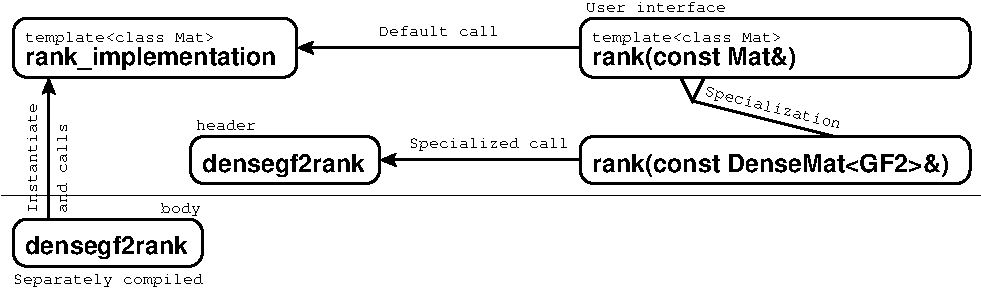
\includegraphics[width=\textwidth]{separate}
\caption{Separate compilation of the rank}\label{fig:sep}
\end{figure}

\begin{remark} 
  Algorithm \ref{alg:sep} has been simplified for the
  sake of clarity. To enable a more user-friendly interface one can
  rename the original function and all its 
  original specializations \texttt{func\_original}; then rename also
  the new interface
% (\texttt{func\_separate}) 
 simply \texttt{func}. 
This allows to keep the legacy interface unchanged. 
\end{remark}

\begin{remark} 
With the classical inline compiler optimizations, the overhead of
calling \texttt{func\_separate} is limited to single supplementary
function call. Indeed all the one line additional methods will be
automatically inlined, except, of course, the one calling the separately
compiled code.
If this overhead is too expensive, it suffices to enclose all the non generic specializations of
``func\_instantiate.hpp'' by a macro test. 
At compile time, the decision to separately
compile or not can be taken according to the definition of this
macro. 
\end{remark}


We show in table \ref{tab:compilation} the gains in compilation time
obtained on two examples from \linbox: the \texttt{examples/\{rank,solve\}.C} algorithms. 
 Indeed, without any specification
 the code has to invoke several specializations depending on
 run-time discovered properties of the input. For instance
 \texttt{solve.C} requires 6 specializations for sparse
 matrices over the Integers or over a prime field, with a sparse
 elimination, or an iterative method, or a dense method, if the matrix
 is small\ldots
\begin{table}[ht]\center
\begin{tabular}{|l||r|r|r||r|r|r|}
\hline
file                      &  real time   &  user time   &  sys. time  &  real time   &  user time   &  sys. time \\
\hline
 & \multicolumn{3}{|c||}{Rank}& \multicolumn{3}{|c|}{Solve}\\
\hline
\texttt{instantiate.o} & 143.43s & 142.47s & 0.90s & 171.62s & 170.42s & 1.12s\\
\texttt{\{rank,solve\}.o} & \bf 18.58s & \bf 18.26s & \bf 0.30s & \bf 23.13s & \bf 22.80s & \bf 0.32s\\
\texttt{link} & 0.80s & 0.64s & 0.15s & 0.85s & 0.70s & 0.14s\\
\hline
\texttt{Sep. comp. total} & 162.81s & 161.37s & 1.35s & 195.60s & 193.92s & 1.58s\\
\hline
\texttt{Full comp.} & 162.02s & 160.47s & 1.21s & 191.47s & 189.52s & 1.40s\\
\hline
\hline
\texttt{speed-up} & 8.4 & 8.5 & 2.7 & 8.0 & 8.1 & 3.0\\
\hline
\end{tabular} 
\caption{linbox/examples/\{rank,solve\}.C compilation time on an AMD
  Athlon 3600+, 1.9GHz, with gcc-4.5 -O2. \texttt{instantiate.o} contains to the separately compiled
  instantiations (e.g. densegf2rank in figure \ref{fig:sep});
  \texttt{\{rank,solve\}.o} contains to the user interface and generic
  implementation compilation; \texttt{link} corresponds to the linking
  of both \texttt{.o} and the library; \texttt{Full comp.} corresponds
  to the compilation without the separate
  mechanism.}\label{tab:compilation}
\end{table}


\begin{table}[ht]\center
\begin{tabular}{|l||r|r|r||r|r|r|}
\hline
file                      &  real time   &  user time   &  sys. time  &  real time   &  user time   &  sys. time \\
\hline
 & \multicolumn{3}{|c||}{Rank}& \multicolumn{3}{|c|}{Solve}\\
\hline
\texttt{instantiate.o} & 46.36s & 44.47s & 1.33s & 67.32s & 63.16s & 2.20s\\
\texttt{separate.o} & \bf 9.51s & \bf 9.13s & \bf 0.30s & \bf 9.88s & \bf 9.38s & \bf 0.30s\\
\texttt{separate} & 0.55s & 0.34s & 0.07s & 0.97s & 0.72s & 0.08s\\
\hline
\texttt{Sep. comp.} & 56.42s & 53.94s & 1.70s & 78.17s & 73.26s & 2.58s\\
\hline
\texttt{Full comp.} & 50.60s & 46.88s & 1.90s & 70.42s & 65.55s & 2.42s\\
\hline
\hline
\texttt{speed-up} & 5.0 & 5.0 & 5.1 & 6.5 & 6.5 & 6.4\\
\hline
\end{tabular} 
\caption{linbox/examples/\{rank,solve\}.C compilation time on an intel
  Xeon E5345, 2.33GHzAMD, with icc-11.1 -O2.}\label{tab:icccomp}
\end{table}


\section{Conclusion}

Proposal ``Parallel building blocs'' for Linbox
- separation of concern between computer algebra and parallelism
- allows several parallel implementations
- not so intrusive with new C++XX standard
- Which STL algorithms ?


High performance multicore in Linbox is a short term
objective
- pbb: data parallel construction with dynamic scheduling
- Xkaapi (for a next meeting): task parallelism with few
intrusion in the code (no more ``SHARED'' type).
- scheduling is mature

Distributed Linbox
- Means a way to serialize data
- Iso allocation + communication of memory pages; Few code intrusion
- What about the coherency protocol ?

%{\par\noindent\bf Acknowledgment}\\
\section*{Acknowledgment}
We thank the \linbox group and especially Brice Boyer, Pascal Giorgi,
Erich Kaltofen, Dan Roche, Brian Youse for many useful discussions 
in particular during the recent \linbox developer meetings in
Delaware and Dublin.

\bibliographystyle{plain}
\bibliography{icms} 
\end{document}
